\section{Data Exploration}
\label{section:data_exploration}

At this point the data from the ask.fm site has been analysed, extracted and classified. The next step is to explore the data and get a better understanding of its contents and quality. It could be argued that an exploration of the data would have been better performed before it was classified. However, because of the simplicity of the structure of the data used in this research project it was decided that there was nothing to be gained in performing the exploration first. In this section, the structure of the data is briefly described before giving details of the exploration performed and also the finding. Finally the quality of the data is reviewed.

\subsection{Data Description}
In the previous section the classification process was described where each question was classified as bullying, not bullying or discard. This classification attribute, along with the anonymous question identify was imported back into the MySQL database to allow further exploration of the data and for future access. A simple view of the database schema is shown in Figure \ref{fig:chapter4:thesis_schema}. This is the view of the schema automatically generated by the MySQL Workbench Tool.

\begin{figure}[htbp]
	\centering
	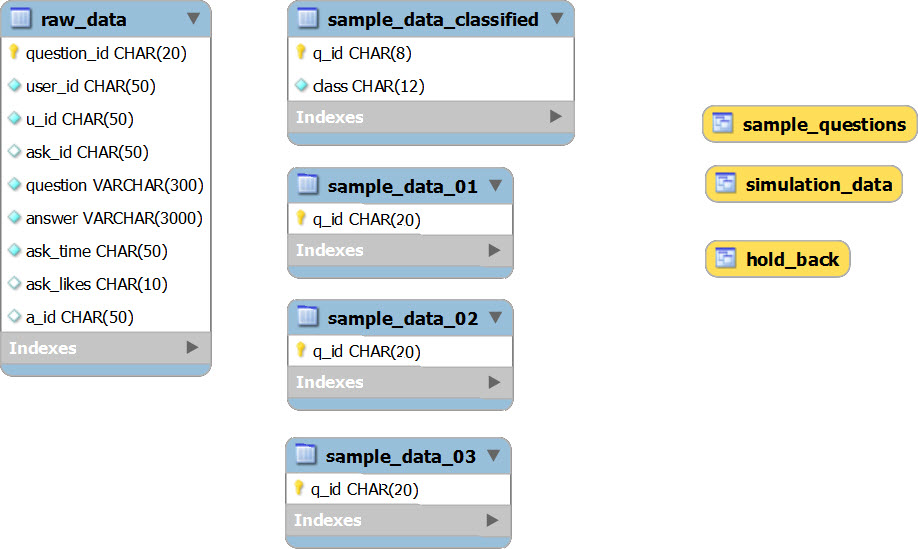
\includegraphics[width=0.85\textwidth]{Figures/Chapter4/thesis_schema.jpg}
	\caption[View of the thesis schema]{A simple representation of the thesis schema.}
	\label{fig:chapter4:thesis_schema}
\end{figure}

To recap, the \verb|raw_data| table is the all of data as extracted from the HTML files of each of users whose questions were scraped earlier. The \verb|sample_data_01| table contains the anonymous question ids, representing 10\% of all questions, to be used for generation of the model and the \verb|sample_data_classified| table is the same list of the anonymous question ids and their classification label. From these tables the \verb|sample_questions| view was created to allow easy access to the primary data attributes. Over the course of the data exploration exercise many views of the data were created. Table \ref{tab:chapter4:rawdata} provides a brief description of each of the attributes in the \verb|raw_data| table. The only other attribute shown that is not included in this table is the \verb|class| attribute which holds the classification of whether the question is bullying or not bullying.

\begin{table}[h]
\centering
\caption[Description of raw\_data table]{Table describing the purpose of each attribute in the raw\_data table.}
\label{tab:chapter4:rawdata}
\begin{tabular}{ll}
	\toprule
    \textbf{Attribute}    & \textbf{Description}                   \\
    \midrule
    question\_id & The ask.fm question id        \\
    q\_id        & The anonymous question id     \\
    user\_id     & The ask.fm id of the user     \\
    u\_id        & The anonymous id of the user  \\
    ask\_id      & The ask.fm id of the asker    \\
    a\_id        & The anonymous id of the asker \\
    question     & The question                  \\
    answer       & The answer                    \\
    ask\_time    & When the question was asked   \\
    ask\_likes   & The number of likes received  \\
    \bottomrule
    \end{tabular}
\end{table}

\subsection{Data Quality}
Upon review of the data in the \verb|raw_data| table, it was immediately apparent that there were some minor issues with the text in the question and answers field. As initially only the questions would be used this was where effort was concentrated when determining data quality.

\begin{itemize}

	\item Questions with only images as answers appeared empty \\
	These are of no use in the automated classification of the question. There is no feasible way to replace a picture with text so these records will be removed from the dataset.
	\item Records with only numerical answers \\
	These will be of little value when trying to establish what features help identify text as bullying so will also be removed. 
	\item Records where part or all of the text was not English. \\
	Every effort was made though to only select English speaking users. There was little evidence of questions in languages other than English so no further investigation or processing is required.
	\item Records where non ASCII characters were used \\
	There was some evidence of the use of non ASCII characters. To simplify and standardise word tokens non ASCII characters will either be removed or replaced with their ASCII equivalent.
	\item Slang words, emoticons and abbreviations \\
	Slang words are usually very descriptive in nature and will be useful when developing the classification model. There is no need to attempt to identify, remove or replace these words. Emoticons are typically inconsistently used and often the same emoticon sentiment can be characterised in many different ways. Emoticons will be removed. To preserve sentence integrity, abbreviations should be replaced with the correct word token.
	\item Repeated characters \\
	Sometimes certain letters in words are repeated to emphasise the word. Where appropriate these repeated letters should be removed to reduce the number of distinct word tokens in the corpus.
	
\end{itemize}

These issues will further investigated and handled in Section \ref{section:data_prepatation}.

\subsection{Data Exploration}

Now that there is a basic understanding of the data it will be explored in more detail by visualising some of the key attributes. There is not actually much exploration required as the dataset is so simple. The first aspect to be examined is the number of records, questions, each user contributed to the total dataset and to ensure that when this total number of records was partitioned into the three separate data blocks that the approximate user to question ratios were maintained. It is also important to ensure that an average of 10\% of each users records were allocated to the block of data to be used for modelling. The total number of records per user is shown in the top chart in Figure \ref{fig:chapter4:user_distributions}. The criteria for user selection was that each user should have answered at least 1,000 question and no more than approximately 4,000. As can be seen there is a good distribution of the numbers of questions and, although the top three number of questions answered are greater than 4000, it can be said that this criterion has been met. The middle and bottom charts show the count of records each user contributed to the training dataset and the percentage of their total number of questions that this represents respectively. Although it can be seen that the percentages, at the extremes, vary between approximately 8.3\% and 11.7\%, at an overall average value of 9.92\% and a standard deviation of 0.7\% this distribution is acceptable.

\begin{figure}[htbp]
	\centering
	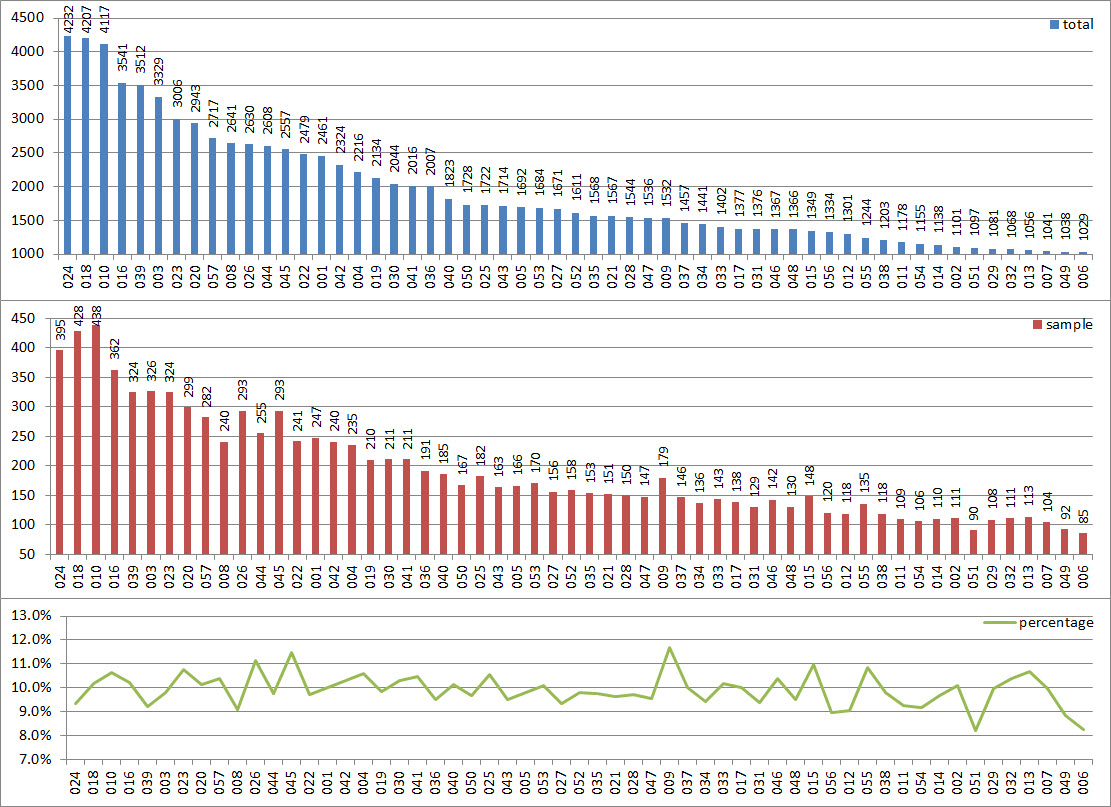
\includegraphics[width=1\textwidth]{Figures/Chapter4/user_distributions.jpg}
	\caption[Distribution of user records]{Distribution of users records showing the total number per user and the number and percentage of each users records in the training dataset}
	\label{fig:chapter4:user_distributions}
\end{figure}

Next the sample questions that will be used for modelling are further explored. The first two attributes to be examined are the distribution of the questions, between the bullying and not bullying classes, and an analysis of the number of anonymous questions that are asked. As shown in Figure \ref{fig:chapter4:class_distribution} approximately 1 question in every 7 was classified as bullying and that slightly less than 1\% of all question were identified as being not suitable for inclusion and could be discarded. The ratio of bullying question to not bullying questions is in line with figures obtained from other research projects in this area. In total 1,644 questions were classified as bullying.

\begin{figure}[htbp]
	\centering
	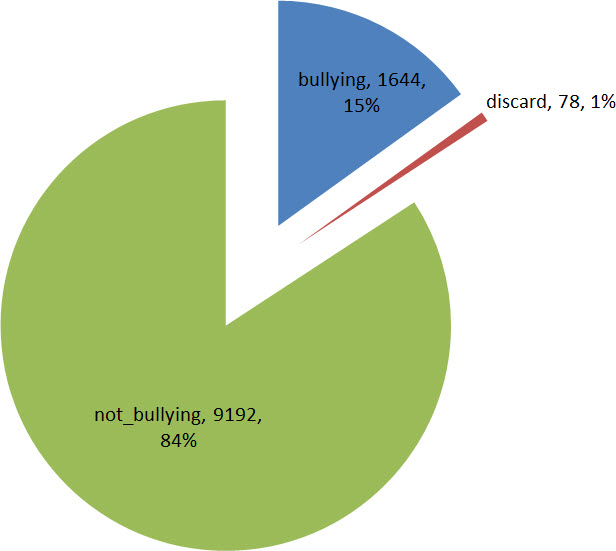
\includegraphics[width=0.55\textwidth]{Figures/Chapter4/class_distribution.jpg}
	\caption[Class Distribution of Sample Questions]{Class Distribution of Sample Questions}
	\label{fig:chapter4:class_distribution}
\end{figure}

\begin{figure}[htbp]
	\centering
	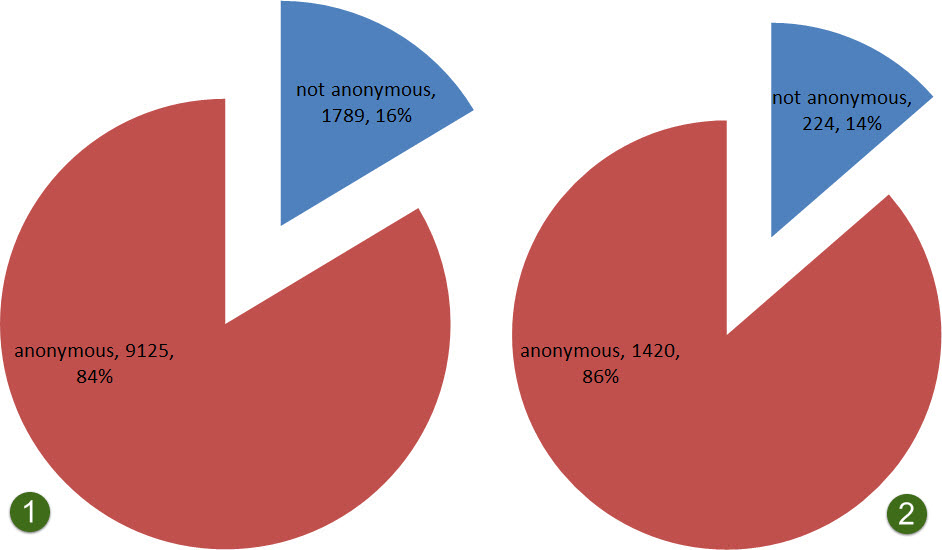
\includegraphics[width=0.8\textwidth]{Figures/Chapter4/anonymous_distribution.jpg}
	\caption[Sample Questions asked Anonymously]{Ratio of all questions asked anonymously (1) and ratio of questions classified as bullying asked anonymously (2)}
	\label{fig:chapter4:anonymous_distribution}
\end{figure}

The number of questions that were asked anonymously, and also the number of questions classified as bullying that were asked anonymously was also examined. There are 10,914 records in the sample questions dataset and it was noticed immediately that the percentage of anonymous questions that are asked was extremely high at 84\%. Unsurprisingly the number of anonymous questions that were classified as bullying was also very high at 86\% as shown on the right hand side of Figure \ref{fig:chapter4:anonymous_distribution}. Of the 1,644 questions that were classified as bullying 1,420 were asked anonymously and 224 were not asked anonymously.

Table \ref{tab:chapter4:not_anon_bullying} takes a closer look at the 224 question that were not asked anonymously. Two-thirds of the questions that were not asked anonymously were single questions asked by a user. Including instances where an identifiable user asked two questions that were classified as bullying, nearly 91\% of all bullying questions that were not asked anonymously were asked by a user who only asked one or two bullying questions. In total 5 users asked three or more anonymous bullying questions. In each case the bullying questions were asked to the same user. For example, the user identified by id \verb|4145| asked user \verb|57| seven questions, out of a total of thirty seven, that were classified as bullying. This suggests a familiarity between the two users and perhaps the questions are not bullying but just banter between two friends. However, as the total number of questions in this category are low, and the primary goal of this research is solely the identification of bullying posts, such considerations are not in scope now but could possibly be included in any future work.

\begin{table}[h]
\centering
\caption[Bullying questions that are not anonymous]{Table showing the break down of questions that were not asked anonymously by the id of the asker.}
\label{tab:chapter4:not_anon_bullying}
\begin{tabular}{rrrc}
	\toprule
    \textbf{Questions Asked} & \textbf{\# Users} & \textbf{\# Questions} & \textbf{Percentage}            \\
    \midrule
	7	& 1		&	7	&	3.1\%	\\
	4	& 2		&	8	&	3.6\%	\\
	3	& 2		&	6	&	2.7\%	\\
	2	& 27	&	54	&	24.1\%	\\
	1	& 149	&	149	&	66.5\%	\\
    \bottomrule
    \end{tabular}
\end{table}

The average length of questions classified as bullying and those classified as not bullying was analysed. As shown in Figure \ref{fig:chapter4:avg_question_len} the average length of a question that was classified as bullying is nearly 19\% longer than a question that is not. However with an overall average length of 42.3 with a standard deviation of 42.2 this difference in question lengths does not appear to be of great importance.

\begin{figure}[htbp]
	\centering
	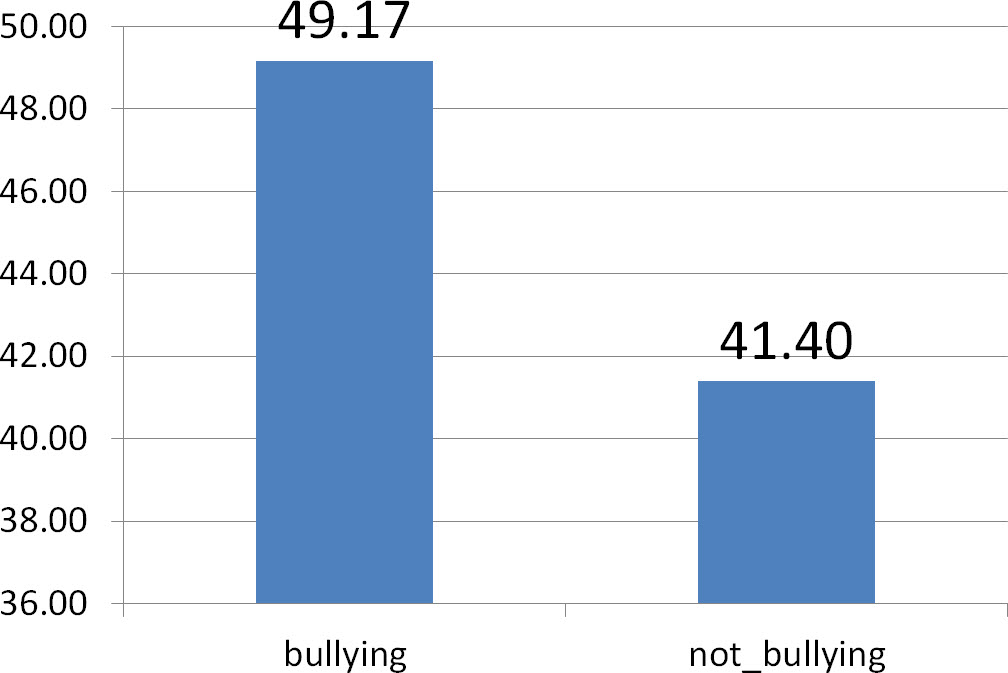
\includegraphics[width=0.5\textwidth]{Figures/Chapter4/avg_question_len.jpg}
	\caption[Average question length per class]{The average question length for questions classed as bullying and those that are not.}
	\label{fig:chapter4:avg_question_len}
\end{figure}

The corpus of distinct words, and the count of the number of times each word was used, was then examined. A simple Python script was developed to identify all distinct words in the corpus and also count the number of occurrences of each word. Unique words, or tokens, that were at least 2 characters long were considered. There were 12,162 distinct string tokens that met this criterion with 85988 tokens in total. The average word occurrence frequency was 7.07 but with a massive standard deviation of 69.38. The questions were then divided into not bullying and bullying corpora, and the analysis performed again. Table \ref{tab:chapter4:word_count} shows the twenty most frequently occurring words for all questions, not bullying questions and bullying questions. A quick glance at the table shows that when these words are considered there is no obvious discernible difference between the words in the not bullying questions corpus and the words in the bullying questions corpus. When comparing the top twenty words in the not bullying and bullying classes it can be seen that four in every five words, or 80\%, appear in both lists.

\begin{table}[h]
\centering
\caption[Distinct word counts]{Table showing distinct word counts for all questions and separately for not bullying and bullying questions}
\label{tab:chapter4:word_count}
\begin{tabular}{lrlrlr}
	\toprule
	\multicolumn{2}{c}{\textbf{Total}} & \multicolumn{2}{c}{\textbf{Not Bullying}} & \multicolumn{2}{c}{\textbf{Bullying}}\\
	\cmidrule(r){1-2}
	\cmidrule(r){3-4}
	\cmidrule(r){5-6}
    \textbf{Word} & \textbf{Count} & \textbf{Word} & \textbf{Count} & \textbf{Word} & \textbf{Count}           \\
    \midrule
	you		& 5399	&	you		&	4492	&	you		&	907	\\
	your	& 1759	&	what	&	1520	&	your	&	370	\\
	the		& 1716	&	the		&	1488	&	and		&	313	\\
	to		& 1701	&	do		&	1422	&	to		&	283	\\
	what	& 1657	&	to		&	1418	&	the		&	228	\\
	do		& 1573	&	your	&	1389	&	are		&	223	\\
	and		& 1345	&	and		&	1032	&	of		&	172	\\
	is		& 1114	&	is		&	986		&	have	&	158	\\
	are		& 1076	&	are		&	853		&	do		&	151	\\
	like	& 895	&	like	&	753		&	like	&	142	\\
	in		& 816	&	in		&	687		&	so		&	137	\\
	of		& 772	&	on		&	612		&	what	&	137	\\
	have	& 726	&	of		&	600		&	in		&	129	\\
	on		& 714	&	would	&	571		&	is		&	128	\\
	would	& 650	&	have	&	568		&	with	&	127	\\
	so		& 632	&	that	&	517		&	me		&	126	\\
	that	& 610	&	if		&	497		&	on		&	102	\\
	it		& 569	&	so		&	495		&	ur		&	102	\\
	now		& 561	&	who		&	489		&	how		&	97	\\
	who		& 555	&	how		&	464		&	that	&	93	\\
    \bottomrule
    \end{tabular}
\end{table}

This word count exploration was performed again. In addition to only selecting words that were at least 2 characters long, all English stop words defined in the Python Natural Language Tool Kit were removed. Now, whilst there are still 12,044 distinct tokens, overall there are only 49,942 token instances, a 42\% decrease, with an average word occurrence of only 4.15. The results of this word count analysis is shown in Table \ref{tab:chapter4:word_count_nostop}.  Although there is now some better differentiation between the not bullying and bullying questions, there are still 12 common words in the top twenty words of each category. This suggests that building a model to predict the class of questions using word counts alone will not be predictive enough and that maybe additional strategies will need to be considered.

\begin{table}[h]
\centering
\caption[Distinct word counts, no stop words]{Table showing distinct word counts for all questions and separately for not bullying and bullying questions with stop words removed}
\label{tab:chapter4:word_count_nostop}
\begin{tabular}{lrlrlr}
	\toprule
	\multicolumn{2}{c}{\textbf{Total}} & \multicolumn{2}{c}{\textbf{Not Bullying}} & \multicolumn{2}{c}{\textbf{Bullying}}\\
	\cmidrule(r){1-2}
	\cmidrule(r){3-4}
	\cmidrule(r){5-6}
    \textbf{Word} & \textbf{Count} & \textbf{Word} & \textbf{Count} & \textbf{Word} & \textbf{Count}           \\
    \midrule
	like	& 895	&	like	&	753	&	like	&	142	\\
	would	& 650	&	would	&	571	&	ur		&	102	\\
	don't	& 349	&	think	&	307	&	would	&	79	\\
	think	& 344	&	don't	&	276	&	don't	&	73	\\
	know	& 327	&	know	&	260	&	pic		&	69	\\
	ur		& 323	&	love	&	258	&	know	&	67	\\
	love	& 302	&	:)		&	252	&	get		&	58	\\
	:)		& 294	&	favorite&	245	&	post	&	56	\\
	you're	& 292	&	you're	&	238	&	f**k	&	56	\\
	get		& 285	&	get		&	227	&	you're	&	54	\\
	really	& 261	&	best	&	222	&	want	&	53	\\
	one		& 253	&	ur		&	221	&	i'm		&	52	\\
	favourite& 250	&	one		&	220	&	really	&	50	\\
	i'm		& 238	&	people	&	213	&	see		&	50	\\
	best	& 238	&	really	&	211	&	go		&	50	\\
	go		& 238	&	what's	&	208	&	love	&	44	\\
	people	& 235	&	ever	&	194	&	old		&	42	\\
	ever	& 233	&	thing	&	189	&	bitch	&	42	\\
	what's	& 226	&	go		&	188	&	right	&	40	\\
	want	& 224	&	i'm		&	186	&	ever	&	39	\\
    \bottomrule
    \end{tabular}
\end{table}

A common strategy used in text mining classification is the generation of term n-grams. N-grams have the effect of concatenating together two or more tokens to form new hopefully more predictive tokens. For example the quote \textit{``to be or not to be''} produces the following tri-grams:

\begin{itemize}

	\item to\_be\_or
	\item be\_or\_not
	\item or\_not\_to
	\item not\_to\_be
	
\end{itemize}

Bi-grams, two tokens, and tri-grams, three tokens, word lists were generated from the bullying and not bullying questions examined earlier. As before only words or tokens that were at least two characters long were considered. Word or token frequencies were determined and these results are shown in Tables \ref{tab:chapter4:word_count_bi-gram} and \ref{tab:chapter4:word_count_tri-gram}.

\begin{table}[h]
\centering
\caption[Distinct bi-gram word counts]{Table showing distinct counts of bi-gram tokens for not bullying and bullying questions with and without stop words}
\label{tab:chapter4:word_count_bi-gram}
\begin{tabular}{lrlrlrlr}
	\toprule
	\multicolumn{4}{c}{\textbf{Not Bullying}} & \multicolumn{4}{c}{\textbf{Bullying}} \\
	\cmidrule(r){1-4}
	\cmidrule(r){5-8}
	\multicolumn{2}{c}{\textbf{With Stopwords}} & \multicolumn{2}{c}{\textbf{No Stopwords}} & \multicolumn{2}{c}{\textbf{With Stopwords}} & \multicolumn{2}{c}{\textbf{No Stopwords}} \\
    \midrule
	do\_you			& 959 &	would\_like		 & 74 &	are\_you  &	93 & right\_now		& 28	\\
	what\_is		& 344 &	would\_be		 & 47 &	do\_you   &	72 & wearing\_right	& 20	\\
	are\_you		& 342 &	don't\_know		 & 42 &	you\_have &	42 & post\_pic		& 16	\\
	would\_you		& 318 &	one\_thing		 & 41 &	you\_are  &	40 & don't\_know	& 15	\\
	if\_you			& 259 &	last\_time		 & 40 &	what\_are &	40 & old\_you		& 14	\\
	you\_like		& 246 &	what's\_favorite & 40 &	how\_old  &	37 & cut\_cut		& 8	\\
	is\_the			& 215 &	last\_person	 & 33 &	want\_to  &	31 & post\_picture	& 7	\\
	is\_your		& 198 &	right\_now		 & 32 &	if\_you   &	30 & would\_go		& 6	\\
	your\_favorite	& 184 &	best\_friends	 & 27 &	of\_you   &	30 & dont\_like		& 6	\\
	have\_you		& 179 &	best\_friend	 & 25 &	pic\_of   &	29 & look\_like		& 6	\\
    \bottomrule
    \end{tabular}
\end{table}

Examining the top ten most frequently occurring bi-gram tokens some features are immediately apparent. The first most obvious thing to notice is that where stop words are not removed only three out of the ten not bullying tokens, 30\%, also appear in the bullying list. When compared to the top ten uni-grams, single words tokens, where 80\% of the top ten tokens appears in both lists this represents a possible indicator that bi-grams would be of more use in the classification of unseen questions. When stop words are removed the number of common words fell from six out of ten repeated uni-grams, 60\%, to only two out of 10 or 20\% bi-grams. Also of note is the use of \verb|you|, the second person pronoun. When stop words are not removed \verb|you| is prominent, appearing in six out of the top ten bi-grams in both the not bullying and word bullying lists. Another pronoun, \verb|your|, also appears twice in the not bullying top ten list. However, when stop words are removed \verb|you| does not appear at all in the not bullying top ten and only once in the bullying top ten. This observation flies somewhat in the face of \citet{yin_detection_2009} which mentioned that when reviewing their dataset it was noticed that a lot of the posts classified as harassment contained foul language used in conjunction with pronouns, particularly second person personal pronouns such as ``you'', ``your'' and ``yourself''. An examination of the data from Ask.fm does not, at first sight, corroborate these findings. 

\begin{table}[h]
\centering
\caption[Distinct tri-gram word counts]{Table showing distinct counts of tri-gram tokens for not bullying and bullying questions with and without stop words}
\label{tab:chapter4:word_count_tri-gram}
\begin{tabular}{lrlr}
	\toprule
	\multicolumn{4}{c}{\textbf{Not Bullying}} \\
	\cmidrule(r){1-4}
	\multicolumn{2}{c}{\textbf{With Stopwords}} & \multicolumn{2}{c}{\textbf{No Stopwords}} \\
    \midrule
	what\_is\_your		& 154 &	would\_like\_meet		& 74 \\
	what\_do\_you		& 153 &	people\_think\_you		& 47 \\
	do\_you\_think		& 133 &	favorite\_month\_year	& 42 \\
	what\_is\_the		& 132 &	many\_times\_day		& 41 \\
	do\_you\_like		& 128 &	gift\_would\_like		& 40 \\
	is\_your\_favorite	& 110 &	think\_people\_think	& 40 \\
	if\_you\_could		& 94 &	what's\_longest\_you've	& 33 \\
	what\_would\_you	& 86 &	last\_thing\_made		& 32 \\
	was\_the\_last		& 79 &	anyone\_right\_now		& 27 \\
	you\_like\_to		& 76 &	made\_happy\_today		& 25 \\
    \bottomrule
    \end{tabular}
\begin{tabular}{lrlr}
	\toprule
	\multicolumn{4}{c}{\textbf{Bullying}} \\
	\cmidrule(r){1-4}
	\multicolumn{2}{c}{\textbf{With Stopwords}} & \multicolumn{2}{c}{\textbf{No Stopwords}} \\
    \midrule
	what\_are\_you		& 30 &	wearing\_right\_now		& 20 \\
	how\_old\_are		& 24 &	cut\_cut\_cut			& 7 \\
	are\_you\_wearing	& 21 &	last\_person\_kissed?	& 5 \\
	wearing\_right\_now	& 20 &	whoever\_likes\_thinks	& 4 \\
	you\_wearing\_right	& 20 &	see\_window\_post		& 4 \\
	old\_are\_you		& 13 &	window\_post\_pic		& 4 \\
	have\_you\_ever		& 11 &	slept\_ex\_bf			& 3 \\
	of\_you\_and		& 10 &	shannon\_slept\_ex		& 3 \\
	post\_pic\_of		& 10 &	likes\_thinks\_you're	& 3 \\
	do\_you\_have		& 9  &	ex\_bf\_max				& 3 \\
    \bottomrule
    \end{tabular}
\end{table}

An examination of the tri-gram tokens in all categories showed that the top ten most frequently occurring tokens were all unique. Expanding this type of comparison to the top fifty tokens, it was found that when stop words were included three out of every ten tokens, or 30\%, appeared on both the bullying and not bullying lists. Expanding this to the top 100 tokens the repetition fell further to between 24\% and 20\% respectively. Examining next the tri-gram tokens where the stop words had been removed was even more revealing. Only two of the top one hundred not bullying tokens appeared anywhere in the bullying list. In the other direction none of the top 67 bullying tokens appeared anywhere in the top one hundred not bullying tokens. The reason the top 67 bullying tokens were chosen is because after these all tokens only had a frequency of one. Expanding the search to include all not bullying and bullying tri-grams, where the stop words had been removed, showed that only 57 tokens appeared in both lists. This represents 57 out of 21031 not bullying tri-grams, approximately 0.27\%, and 57 out of 5858 bullying tri-grams or 0.97\%. This finding would further support the suggestion that tri-gram tokens should prove to be very good predictors when it comes to developing the models.

One final set of measurements worth considering is the count of distinct tokens in each word list generated and also the average number of times each occurred. This data is summarised in Table \ref{tab:chapter4:word_distribution}. The data is divided into three sections. The first section describes the dataset when all the tokens are considered together. The second describes the not bullying data and the third the bullying data. As previously mentioned there were 12,162 unique uni-grams with 10,514 occurring in the not bullying dataset and 3,598 occurring in the bullying dataset. Delving a little deeper into this information it was discovered that of the 10,514 not bullying tokens 8,238 of these only occurred in the not bullying set showing that over 78\% of these tokens would be good predictors of a not bullying question. Taking the 3,598 bullying token it was seen that 1,575 of these tokens, or approximately 44\%, only occurred in the bullying list. Taking bi-gram tokens next, the percentages of distinct tokens used in either the not bullying dataset or the bullying data set rise to 97\% and 73\% respectively. This diverging of the common words between the two datasets continues all the way up to the tri-gram tokens with stop words removed where, as previously seen, over 99\% of the tokens in each dataset are unique. 

\begin{table}[h]
\centering
\caption[Unique tokens, total count and average frequency]{Table showing the number of distinct tokens in each dataset as well as the total token counts and average frequencies}
\label{tab:chapter4:word_distribution}
\begin{tabular}{lrrr}
	\toprule
	{\textbf{Token}} 		& {\textbf{Unique}} & {\textbf{Total}} & {\textbf{Average}}  \\
	{\textbf{description}}	& {\textbf{Tokens}} & {\textbf{Count}} & {\textbf{Frequency}}  \\
    \midrule
    \midrule
    \multicolumn{1}{l}{\textbf{All Words}} \\
	\cmidrule(l){1-1}
	Uni-Grams					& 12162 &	85988	& 7.1 \\
	Bi-Grams					& 41012 &	75128	& 1.8 \\
	Tri-Grams					& 51111 &	64983	& 1.3 \\
	Uni-Grams No Stop Words		& 12044 &	49942	& 4.1 \\
	Bi-Grams No Stop Words		& 31370 &	39125	& 1.2 \\
	Tri-Grams No Stop Words		& 27106 &	29567	& 1.1 \\
    \midrule 
    \midrule
    \multicolumn{1}{l}{\textbf{Not Bullying}} \\
	\cmidrule(l){1-1}
	Uni-Grams					& 10514 &	70722	& 6.7 \\
	Bi-Grams					& 33665 &	61557	& 1.8 \\
	Tri-Grams					& 40913 &	52981	& 1.3 \\
	Uni-Grams No Stop Words		& 10397 &	40831	& 3.9 \\
	Bi-Grams No Stop Words		& 25204 &	31706	& 1.3 \\
	Tri-Grams No Stop Words		& 21391 &	23604	& 1.1 \\
    \midrule
    \midrule 
    \multicolumn{1}{l}{\textbf{Bullying}} \\
	\cmidrule(l){1-1}
	Uni-Grams					& 3598 &	15208	& 4.2 \\
	Bi-Grams					& 9979 &	13565	& 1.4 \\
	Tri-Grams					& 11086 &	11998	& 1.1 \\
	Uni-grams No Stop Words		& 3489 &	9053	& 2.6 \\
	Bi-Grams No Stop Words		& 6847 &	7413	& 1.1 \\
	Tri-Grams No Stop Words		& 5858 &	5959	& 1.0 \\
    \bottomrule
    \end{tabular}
\end{table}

Next, the distribution of the tokens is further examined and visualised but from Table \ref{tab:chapter4:word_distribution} it is clear to see that the average frequency of each token falls from 7.1 for all uni-grams tokens to 4.1 for uni-grams where stop words have been removed all the way down to nearly a 1:1 ratio for bullying tri-grams where stop words are removed. This shows that very few tokens appear more than once in this tri-gram dataset. This observation suggests that a model based solely on these tri-gram tokens may, in fact, be over trained and would not generalise well to unseen data. This contradicts the earlier suggestion that tri-grams would be good predictors and must be taken into consideration and examined when models are being developed.

\subsection{Data Visualisation}
To visual the not bullying and bullying classes, word clouds, generated using the IBM Many Eyes tool, were used. Uni-grams were considered first and the results of these word clouds can be seen in Figures \ref{fig:chapter4:not_bullying_wordcloud},  \ref{fig:chapter4:bullying_wordcloud}.  When generating the visualisations only the fifty most frequently occurring words were used. It is very clearly seen that \verb|you| dominates both word clouds.


\begin{figure}[!htb]
	\centering
	
\includegraphics[width=0.8\textwidth]{Figures/Chapter4/not_bullying_wordcloud.jpg}
	\caption[Word cloud of not bullying words]{Word cloud of the 50 most frequently occurring words in questions classified as not bullying}
	\label{fig:chapter4:not_bullying_wordcloud}
\end{figure}

\begin{figure}[!htb]
	\centering
	
\includegraphics[width=0.8\textwidth]{Figures/Chapter4/bullying_wordcloud.jpg}
	\caption[Word cloud of bullying words]{Word cloud of the 50 most frequently occurring words in questions classified as bullying}
	\label{fig:chapter4:bullying_wordcloud}
\end{figure}

The exercise was then repeated with the uni-gram tokens where the NLTK stop words had been removed. The two word lists were loaded onto the Many Eyes website and visualised using the same settings as before. Figures  \ref{fig:chapter4:not_bullying_wordcloud_filtered} and \ref{fig:chapter4:bullying_wordcloud_filtered} show the results. It is immediately obvious that the words maps now appear more balanced with a better distribution of word weights across the images. Even so some words, for example \verb|like|, \verb|would|, \verb|don't| and \verb|know|, are still prominent in both classes. It was also observed that some stop words, for example \verb|you|, were still appearing in the word clouds when the token should have been removed. After some investigation it was discovered that the NLTK did not removed stop words where there was an adjacent punctuation character, for example \verb|you!|. These punctuation characters appear to have been striped when the data was loaded into Many Eyes explaining why they are still seen.  

\begin{figure}[!htb]
	\centering
	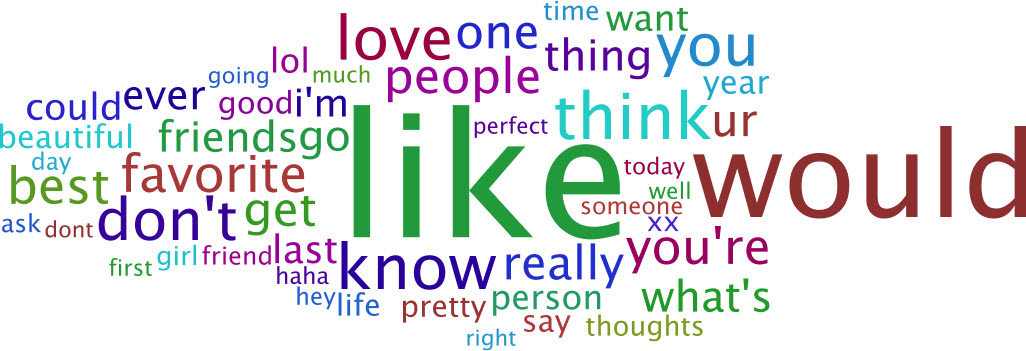
\includegraphics[width=0.8\textwidth]{Figures/Chapter4/not_bullying_wordcloud_filtered.jpg}
	\caption[Filtered word cloud of not bullying words]{Filtered word cloud of the 50 most frequently occurring words in questions classified as not bullying with stop words filtered out}
	\label{fig:chapter4:not_bullying_wordcloud_filtered}
\end{figure}

\begin{figure}[!htb]
	\centering
	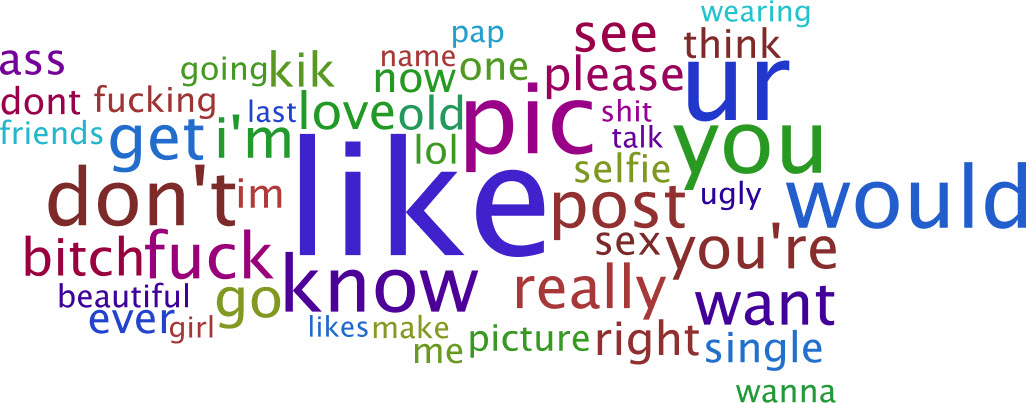
\includegraphics[width=0.8\textwidth]{Figures/Chapter4/bullying_wordcloud_filtered.jpg}
	\caption[Filtered word cloud of bullying words]{Filtered word cloud of the 50 most frequently occurring words in questions classified as bullying with stop words filtered out}
	\label{fig:chapter4:bullying_wordcloud_filtered}
\end{figure}

Whilst the word clouds present a nice way of visualising the frequencies of words in each of the categories, to generate a cloud for all the permutations already highlighted would be very time consuming. Also, any analysis performed on them would be subjective. For example, in Figure \ref{fig:chapter4:bullying_wordcloud_filtered} which word is more prominent \verb|ur| or \verb|pick|. A better way to visualise how the frequencies of words, or tokens, are distributed across each dataset is shown in Figure \ref{fig:chapter4:word_frequencies}. These three graphs shown the normalised word frequencies distributions for the 250 most frequently tokens for all tokens, labelled (1) in the diagram, all not bullying tokens, labelled (2) and all bullying tokens. For brevity, in the legend in each graph \textit{A} represents all tokens, \textit{NB} not bullying and \textit{B} bullying. Similarly \textit{BI} represents bi-grams, \textit{TRI} trigrams and \textit{NO} to show that stop words have been removed. So \textit{B\_TRI\_NO} is used to represent bullying tri-grams with stop words removed.



\begin{figure}[!htb]
	\centering
	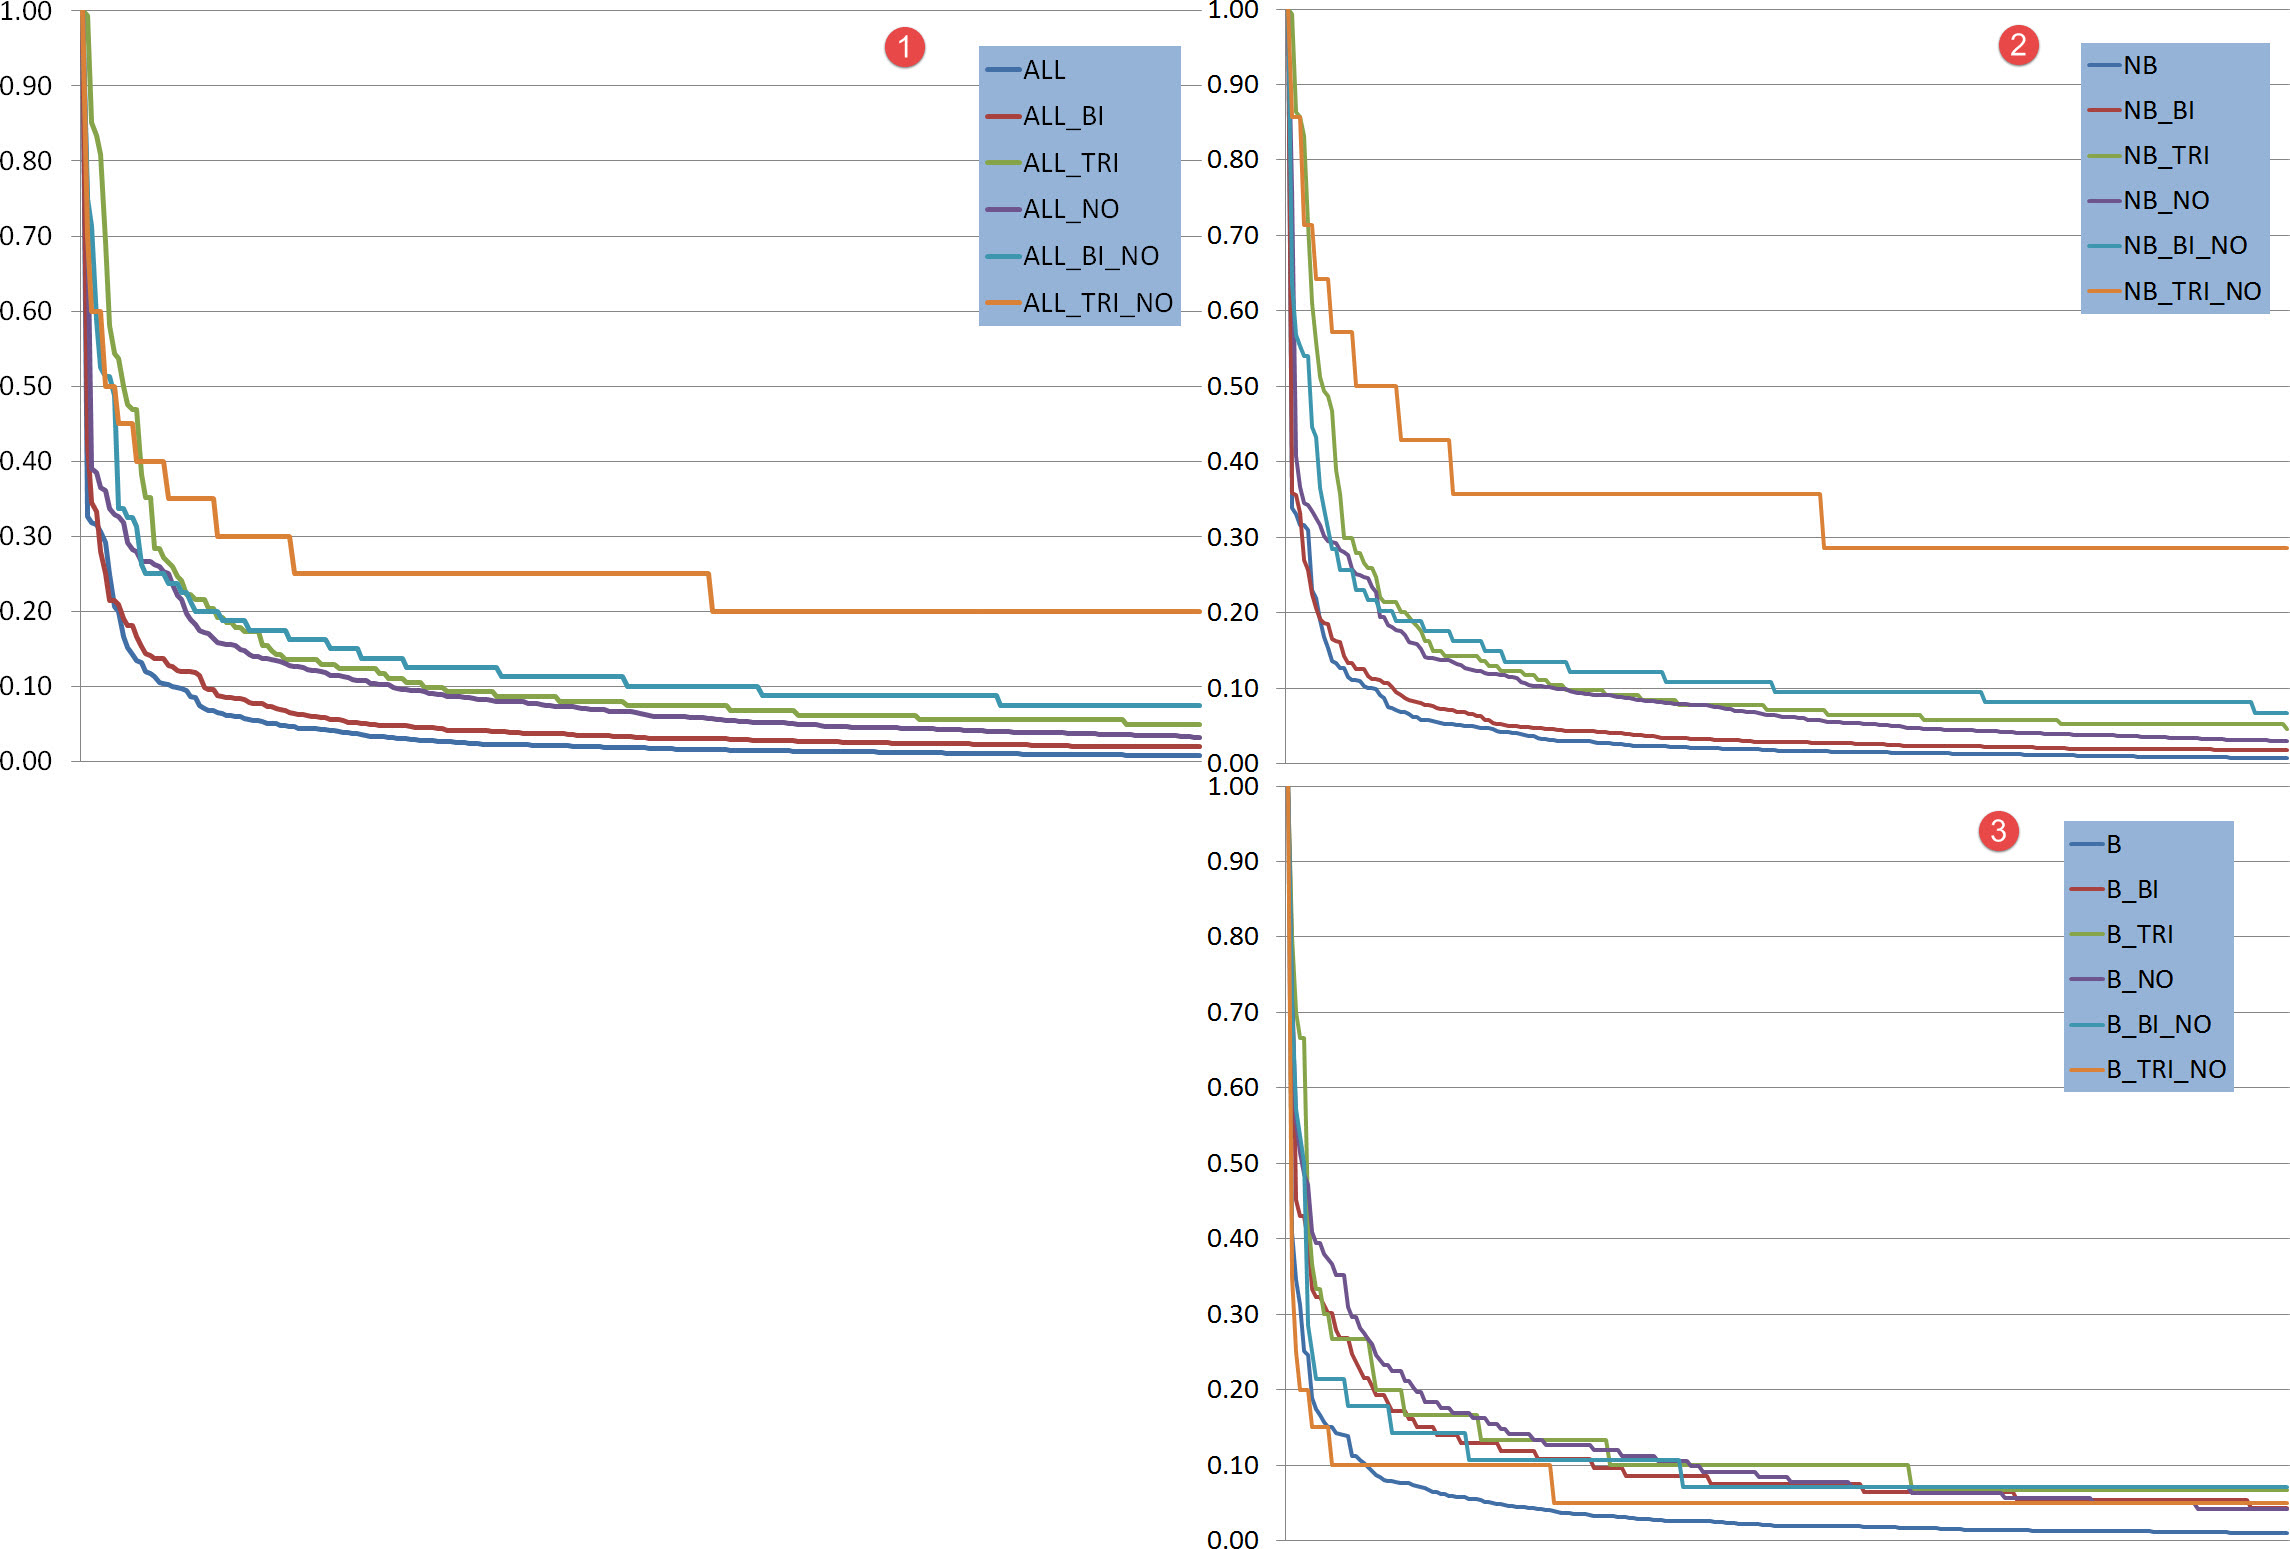
\includegraphics[width=1.0\textwidth]{Figures/Chapter4/word_frequencies.jpg}
	\caption[Normalised distribution of word frequencies]{Graphs showing the normalised word distribution of the different token configurations examined}
	\label{fig:chapter4:word_frequencies}
\end{figure}

Analysing these charts some observations can be immediately noted. Firstly the frequency distribution of tri-gram tokens for all words and for not bullying words, both with stop words removed, have a significantly different shape to all other frequencies. The frequency for not bullying bi-grams is particularly distinctive suggesting maybe that this list is more evenly distributed than the others. It was actually expected that the bullying trigrams would have proven the most evenly distributed dataset. However, the counts of the two most frequency occurring tokens, 20 and 7, when compared to the other frequency counts of 5 or less, meant that the distribution graph for this category fell off faster than any other.



